\documentclass[a4paper]{article}
\usepackage[letterpaper, margin=1in]{geometry} % page format
\usepackage{listings} % this package is for including code
\usepackage{graphicx} % this package is for including figures
\usepackage{amsmath}  % this package is for math and matrices
\usepackage{amsfonts} % this package is for math fonts
\usepackage{tikz} % for drawings
\usepackage{hyperref} % for urls
\usepackage{pdfpages}

\title{Homework 3}
\author{Max Schemitsch}
\date{5/1/2019}

\begin{document}
\lstset{language=Python}

\maketitle

\section{Problem 1}
\subsection{(a)}
To make the code generate 1,000 data points instead of 100, first we make this change in $hw3.problem1\&2.py$:
\begin{lstlisting}[frame=single]
x, y, ytrue = genDataSet(1000)
\end{lstlisting}

\subsection{(b)}
Using $hw3.problem1\&2.py$, the three best values of $k$ are $[1, 3, 5]$.
\subsection{(c)}
The best CV $E_{out}$ is from $k=1$ with 0.0003841882862044138.

\section{Problem 2 (extra credit)}
After 100 experiments, we can see that the best $k$ values are 1 and 3 with this histogram:
\begin{figure}[h]
  \begin{center}
    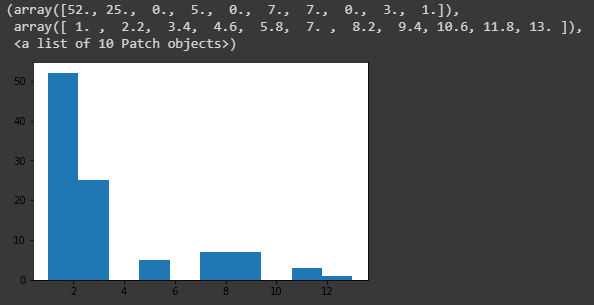
\includegraphics[width=120mm,scale=0.8]{problem2.png}
  \end{center}
\end{figure}

\newpage

\section{Problem 3}
\subsection{(e)}
Using $n\_colors$ equal to 32, 16, and 8 in $hw3.kmeans.img.py$, the picture of myself becomes the following:


\begin{figure}[h]
  \begin{center}
    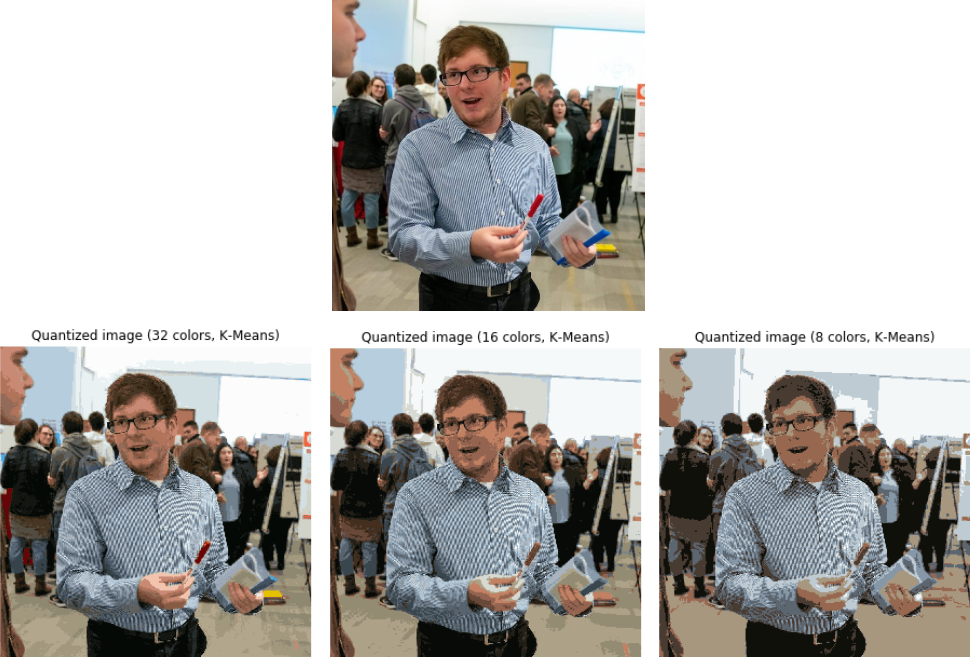
\includegraphics[width=160mm,scale=1]{picsOfMe.png}
  \end{center}
\end{figure}


When the value of $n\_colors$ decreases, the quality of the picture decreases as well. This is because the method is trying to recreate the same image with less and less resources.


This can be useful for a multitude of things, including image compression. Some devices can't handle full-scale images, so being able to reduce color count can help deal with this.


The resulting picture was funny because of how the method dealt with several things. My right hand starts to blend in with my shirt, but throughout all different $k$ values, my shirt looks roughly the same. This is probably because my shirt takes up about one fourth of the picture, making it more prominent.

\newpage

\section{Problem 4}

\subsection{(c)}
Using $hw3.MLP.sol.py$ with 1,000 samples, the best number of neurons is 63. The code output the following:
\begin{lstlisting}[frame=single]
Neurons 63, eta 0.1. Testing set CV score: -2.555428
\end{lstlisting}
\subsection{(d)}
We can see that when adjusting our ETA, an increase seems to make our predictions flat out wrong, a decrease seems to cause a severe over fit. Neither of these are desirable, making an ETA of 0.1 a good starting point. When looking at neurons, we can see for 1,000 samples, that 63 neurons gives us our best cross validation score. After this point, no other amount of neurons gives a better CV error. This makes it apparent that we want a size-able amount of neurons, but not too many neurons. In the next example, with 10,000 samples, the best CV error comes only at 34 neurons. Thus, it seems to be dependent on sample size.
\subsection{(e) (extra credit)}
With 10,000 samples, the best number of neurons is 34. The code output the following:
\begin{lstlisting}[frame=single]
Neurons 34, eta 0.1. Testing set CV score: -0.955031
\end{lstlisting}

\end{document}